\documentclass[a4paper, 12pt]{article}
\usepackage[a4paper,top=1.5cm, bottom=1.5cm, left=1cm, right=1cm]{geometry}
\usepackage{cmap}					% поиск в PDF
\usepackage{mathtext} 				% русские буквы в фомулах
\usepackage[T2A]{fontenc}			% кодировка
\usepackage[utf8]{inputenc}			% кодировка исходного текста
\usepackage[english,russian]{babel}	% локализация и переносы

\usepackage{amsmath}
\usepackage{indentfirst}
\usepackage{longtable}
\usepackage{graphicx}
\usepackage{array}

\usepackage{wrapfig}
\usepackage{siunitx} % Required for alignment
\usepackage{subfigure}
\usepackage{multirow}
\usepackage{rotating}
\usepackage{caption}

\graphicspath{{.}}


\title{\begin{center}Лабораторная работа №2.2.3\end{center}
Измерение удельной теплоёмкости воздуха при атмосферном давлении}
\author{Рожков А. В. \\ Преподаватель Яворский В. А.}
\date{\today}

\begin{document}
    \pagenumbering{gobble}
    \maketitle
    \newpage
    \pagenumbering{arabic}

    \textbf{Цель работы:} измерить коэффициенттеплоп  роводности воздуха при атмосферном давлении в зависимости от температуры.

    \textbf{В работе используются:} цилиндрическая колба с натянутой по оси нитью; термостат; вольтметр и амперметр (цифровые мультиметры); эталонное сопротивление; источник постоянного напряжения; реостат (или магазинсопротивлений).

    \section*{Теоретическая справка}

        \textit{Теплопроводность} — это процесс передачи тепловой энергии от нагретых частей системы к холодным за счёт хаотического движения частиц среды (молекул, атомов и т.п.). В газах теплопроводность осуществляется за счёт  непосредственной передачи кинетической энергии от быстрых молекул к медленным при их столкновениях. Перенос тепла описывается законом Фурье, утверждающим, что плотность потока энергии $\overline{q} = -k \nabla T$, где $k \left[ \dfrac{\text{Вт}}{\text{м} \cdot \text{К}} \right]$ - \textit{коэффициент теплопроводности}.

        Молекулярно-кинетическая теория дает следующую оценку для коэффициента теплопроводности газов:
        \[k \sim \lambda \overline{\nu} \cdot n c_V\]
        С помощью некоторых преобразований мы получаем, что
        \[ Q = \dfrac{2 \pi L}{\ln \dfrac{r_0}{r_1}} k  \cdot \Delta T \]
        \section*{Экспериментальная установка}
        \begin{wrapfigure}{r}{0.4\textwidth}
        \begin{center}
            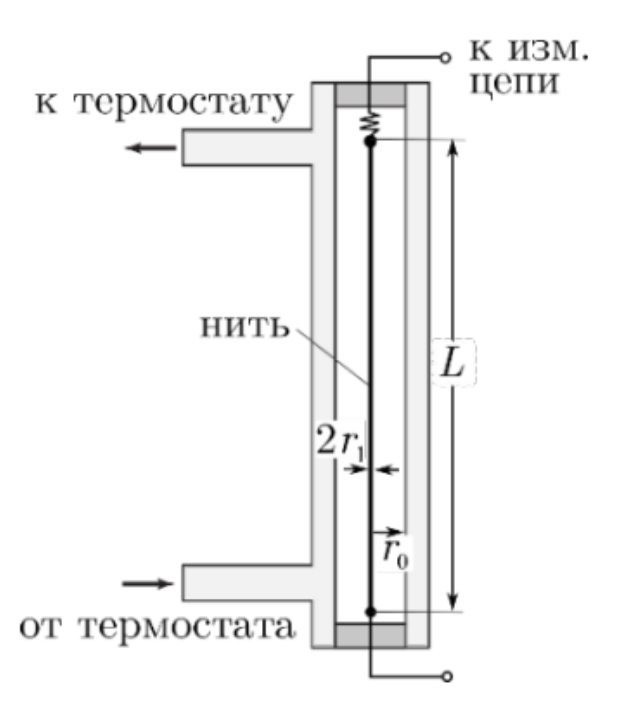
\includegraphics[width = 0.3\textwidth]{pictures/ustanovka.png}
        \end{center}
        \textbf{\caption{Схема установки}}
        \end{wrapfigure}
        Схема установки приведена на рис. 1. На оси полой цилиндрической трубки с внутренним диаметром $2r_0 \sim 1$ см размещена металлическая нить диаметром $2r_1 \sim 0,05$ мм и длиной $L \sim 40$ см (материал нити и точные геометрические размеры указаны в техническом описании установки). Полость трубки заполнена воздухом (полость через небольшое отверстие сообщается с атмосферой). Стенки трубки помещены в кожух, через которых пропускается вода из термостата, так что их температура $t_0$ поддерживается постоянной. Для предотвращения конвекции трубка расположена вертикально.

        Металлическая нить служит как источником тепла, так и датчиком температуры (термометром сопротивления). По пропускаемому через нить постоянному току $I$ и напряжению $U$ на ней вычисляется мощность нагрева по закону Джоуля–Ленца: $Q = UI$, и сопротивление нити по закону Ома: $R = \dfrac{U}{I}$.

        Сопротивление нити является однозначной функцией её температуры $R (t)$.
        Эта зависимость может быть измерена с помощью термостата по экстраполяции мощности нагрева к нулю $Q \rightarrow 0$, когда температура нити и стенок совпадают $t_1 \approx t_0$. Альтернативно, если материал нити известен, зависимость его удельного сопротивления от температуры может найдена по справочным данным.

        На рис. 2 представлена схема электрической установки:
        \begin{figure}
            \begin{center}
                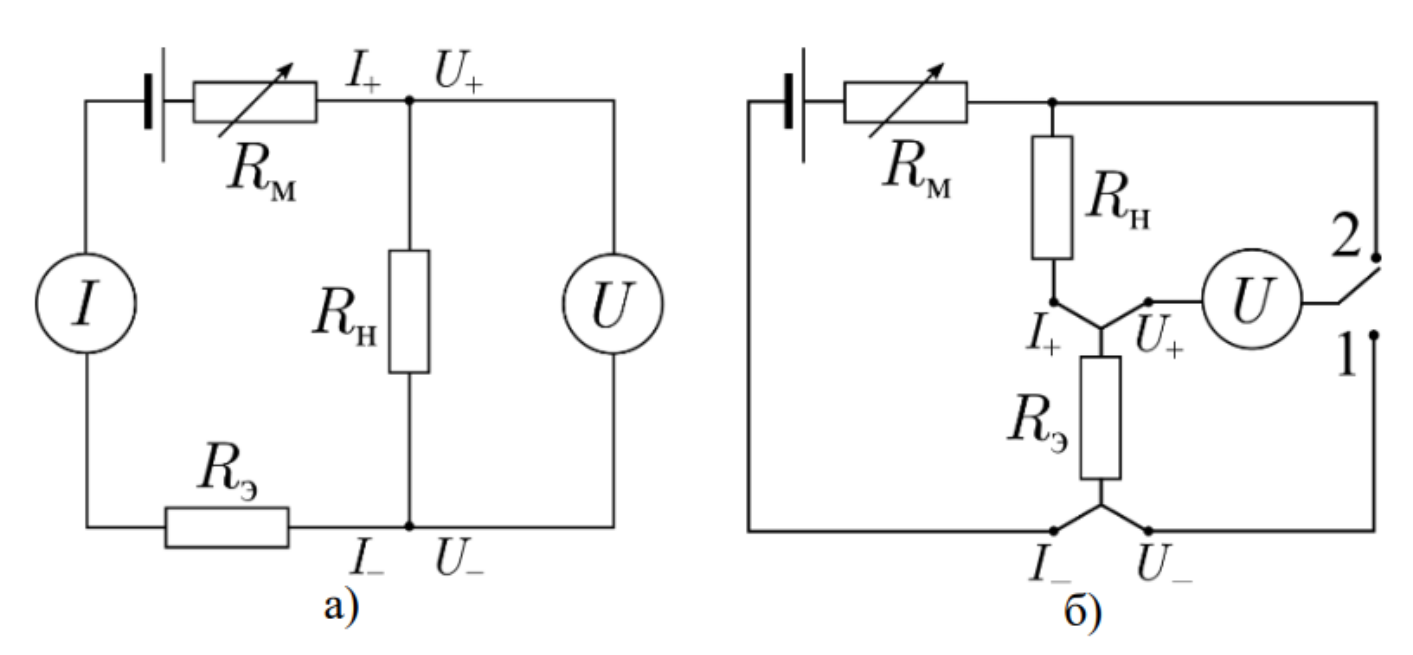
\includegraphics[width = 0.5\textwidth]{pictures/scheme.png}
            \end{center}
            \textbf{\caption{Электрическая схема измерения сопротивления нити и мощности нагрева}}
        \end{figure}

        Схема рис. 2 предусматривает использование одного вольтметра и эталонного сопротивления $R_{\text{э}} \sim 10$ Ом (точное значение $R_{\text{э}}$ и его класс точности указаны в техническом описании установки), включённого последовательно с нитью. В положении переключателя 2 вольтметр измеряет напряжение на нити, а в положении 1 — напряжение на $R_{\text{э}}$, пропорциональное току через нить. Для исключения влияния контактов и подводящих проводов эталонное сопротивление $R_{\text{э}}$ также необходимо подключать в цепь по четырёхпроводной схеме. Ток в цепи в обеих схемах регулируется с помощью реостата или магазина сопротивлений $R_{\text{м}}$, включённого последовательно с источником напряжения.

    \section*{Методика измерений}

        Принципиально неустранимая систематическая ошибка измерения температуры с помощью термометра сопротивления возникает из-за необходимости пропускать через резистор (нить) измерительный ток. Чем этот ток выше, тем с большей точностью будет измерен как он сам, так и напряжение. Однако при этом квадратично возрастает выделяющаяся на  резисторе мощность $Q = UI = I^2R$. Следовательно, температура резистора становится выше, чем у объекта, температуру которого надо измерить. Измерения же при малых токах не дают достаточной точности (в частности, из-за существенного вклада термоэлектрических явлений в проводниках и контактах). Эта проблема решается построением нагрузочной кривой - зависимости измеряемого сопротивления $R$ от выделяющейся в нём мощности $R(Q)$, с последующей экстраполяцией к нулевой мощности $Q \to 0$ для определения сопротивления $R_0 = R(0)$, при котором его температура равна температуре измеряемого объекта. Кроме того, в данной работе измерение нагрузочных кривых позволяет в ходе эксперимента получить температурную зависимость сопротивления нити, так как при $Q \to 0$ температура нити равна температуре термостата ($T \approx T_0$). В исследуемом интервале температур (20-70 $^0C$) зависимость сопротивления от температуры можно с хорошей точностью аппроксимировать линейной функцией:
        \[R(t) = R_{273} \cdot (1 + \alpha t)\]
        где $\alpha = \dfrac{1}{R_{273}} \dfrac{dR}{dT}$ - температурный коэффициент сопротивления материала.

\end{document}
